%Relasjonsalgebra
\chapter{Method}
\label{chapter:method}
This chapter describes the most important decisions and constraints for this
project. Essentially, this chapter describes \emph{what will be done}, however
implementation-specific details are left to chapter
\ref{chapter:implementation}. This chapter is initiated by section
\ref{sect:method:tree_parsing}, where a method for tree parsing is chosen.
Further the method for rewriting the syntax tree is explained in section
\ref{sect:method:ast_rewrite}. Finally we present the target algebra language
(MQL), and the chapter ends with a description of a method for calculating
algebra complexity which will used in chapter \ref{chapter:results} for
comparisons.

\section{Development of a novel translation method}
\textbf{\LARGE TODO:} les over /glimrendeifiser plz.

In section \ref{sect:theory:loop_lifting}, ``Loop Lifting'', the Pathfinder project's method for translating XQuery
queries to relational algebra is presented. As the goal of this Master's thesis is to find a way to translate
queries in this language to MQL, the MARS query language, one possibility would be to modify the Loop Lifting
methodology to produce MQL trees instead. But this modified method would most probably not utilise the full
expressiveness and power of MQL. This lead to the development of a MARS specific method of translation, ``Tainting
Dependencies'', which will be reviewed in full in chapter \ref{chapter:translation}. Another incentive for not
modifying Loop Lifting is that it produces large quite complex operator trees, which lead to unnecessarily
denormalised intermediate results. This will be further discussed in section \ref{sect:disc:res}.


\section{Tree parsing}
\label{sect:implementation:treeparsing}

How we implemented the visitor pattern

\begin{itemize}
  \item Basert p\aa kontekst-sensitiv visitors som beskrevet i teoridelen
  \item Vise UML av greiene
  \item Noen kodeeksempler paa hvordan ting skjer
  \item Greia med en egen rewrite-visitor, som beskrevet i method
\end{itemize}
\section{AST rewriting}
\subsection{Normalizing the syntax tree}
Motivation: simplification
Problem: the XQuery AST is difficult to translate directly
Explain: convert XQuery to something like XQuery core

Forklare hva man skal gjore, ikke hvordan!!

\subsubsection{FLWOR and for-clauses}
\subsubsection{Path predicates}
\subsubsection{Andre ting?}
 
Motivation: simplification
Problem: AST does not correspond to relalg easily
Explain: rewrite multiple predicates for a step expression to a single 
         predicate expression with all subexpressions AND'ed together, ++
         
Kan hende vi ikke kan skrive om predikater til en kombo med AND\ldots hva med
/a/b/c[d = 'cool'][3] ?

\section{Type system}
\label{sect:type_system}
Beskrivelse av det kule typesystemet Som kanskje ikke kommer til \aa~eksistere... =/

Men kan kanskje skrive om hvorfor vi ikke gj\o r det her? Og referere til diskusjon hvor vi sier noe om hvordan
det kan bli gjort\ldots

\section{Target Relational Algebra Language}
\label{sect:method:mql}
Given as premise for this project was the target algebra language. This
algebra is a dialect of classic relational algebra (see section
\ref{sect:theory:relAlg}) developed by FAST Search \& Transfer. The language
is dubbed MQL (Mars Query Language). This section will describe the operators
of this language as well as the indexes they operate on, and will demonstrate
the usage as well as some important traits of this language with a few
examples.

\emph{Note that this section is largely based on documentation provided by FAST which
has been deemed company confidential. }

\subsection{General concepts}
\label{sect:method:mql:indexes}
\label{sect:method:mql:concepts}
All queries for MQL are written as strings with a syntax reminiscient of Lisp
dialects. An example query can be seen in figure \ref{figure:mql:op_example}.

Data is stored in \textit{indexes} rather than in DOM trees. Naturally, this is a prerequisite for efficient
execution of relational algebra on the data. There are two basic index types: \textit{occurence} indexes and
\textit{value} indexes. In the case of an occurence index, a lookup for a term will map the term to the occurences
of this term. In a \textit{value} index, a key (for example document id) is associated to one or more
\textit{values} in the document collection. Lookups in \textit{value} indexes can be combined with lookups in
\textit{occurence} indexes to add data to the result set for the user.
Throughout this chapter and later chapters, any reference to a \textit{valocc}
implies exactly such a hypothetical combination of occurence and value indexes.

The schema of the indexes determins the fields/columns in the result sets from
a lookup, but typically these three fields will be included on a lookup of a
term in the \textit{occurence} index:
\begin{itemize}
  \item Document ID: Internal identifier for the document in which the term
  occurs
  \item Position: The term position in the document (counted by terms, not
  characters or nodes)
  \item Scope: the context of the occurence, e.g \texttt{/a/b}. Note that the
  scope also contains metadata about the \textit{instance} of the scope (this
  is visualised such as this: \texttt{a[1].b[2]}, which reads as ``the first
  instance of \texttt{a} and the second instance of \texttt{b}'')
\end{itemize}
Additionally, a \textit{Value} field can be added by combining the result set
from an \textit{occurence} index with the equivalent result set from a \textit{value}
index. Table \ref{table:method:mql:example_resultset} shows an example result
set from a lookup in a hypothetical \textit{valocc} index.

\begin{table}[!htp]
\begin{center}

\begin{tabular}{| c | c | c | c |}
\hline
\textit{DocumentID} & \textit{Position} & \textit{Scope} & \textit{Value} \\
\hline
1 & 7 & a[1].b[2] & \emph{c} \\ 
\hline
1 & 8 & a[1].b[2] & \emph{c} \\
\hline
1 & 10 & a[1].b[3] & \emph{c} \\ 
\hline
1 & 11 & a[1].b[3] & \emph{c} \\
\hline
\end{tabular}
\caption{Example result set from a lookup in \textit{valocc}}
\label{table:method:mql:example_resultset}
\end{center}
\end{table}

The input for operators are result sets from child operators. The output from
operators is a single result set. Note however that some operators, such as
\texttt{index()} will modify the context for child operators. This feature is
not documented, and the exact mechanics are not known. However their respective
behaviours are described here where applicable.

\subsection{Language syntax}
The syntax of MQL (Mars Query Language) is, as mentioned above, reminiscent of
Lisp dialects. Consider the example in figure \ref{figure:mql:op_example}. This
example will lookup the term ``c'' in the scope \texttt{/a/b} in the index
\textit{valocc}\footnote{The index \textit{valocc} is a hypothetical index
which is simply thought to be a combined lookup in an \textit{occurence}
index and a \textit{value} index}.

\begin{figure}[!h]
\centering
\begin{Verbatim}
index(valocc; 
  scope(/a/b;
    lookup(c)));
\end{Verbatim}
\caption{Simple MQL example}
\label{figure:mql:op_example}
\end{figure}

The syntax for MQL can be described in a condensed form using EBNF notation as
can be seen in figure \ref{figure:mql:ebnf}
\begin{figure}[!h]
\centering
\begin{Verbatim}
OPERATORNAME  ::= IDENTIFIER
OPERATOR      ::= OPERATORNAME "(" PARAMETERLIST? 
                  (";" OPERATORLIST)? ")"
OPERATORLIST  ::= OPERATOR ( "," OPERATOR )*
\end{Verbatim}
\caption{Simplified MQL EBNF}
\label{figure:mql:ebnf}
\end{figure}

Note that \texttt{PARAMETERLIST} has no definition. This production will be
described for each operator, if applicable.

Also note that parameters and child operators are separated by a semicolon. For
example, in the MQL expression \texttt{index(valocc;lookup(hairdresser))} the
\texttt{index()} operator is given one parameter (\texttt{valocc}) and one
child operator (\texttt{lookup(hairdresser)}).

\subsection{Operators}
\label{sect:method:marsOperators}
\subsubsection{Lookup}
\label{sect:method:marsOperators:lookup}
The \texttt{lookup()} operator performs a lookup in the default index (if none
other defined by an \texttt{index()} operator, see
\ref{sect:method:marsOperators:index}). The result set returned from this
operator contains all occurences of the given term, if any. This operator will
use the last index specified by the \texttt{index()} operator, otherwise the
default index. See figure \ref{figure:mql:op_example} for an example of usage. 

\begin{description}
  \item[Input:] none (parameters only)
  \item[Output:] result set with occurences and/or values, depending on index
(see section \ref{sect:method:mql:indexes} above)
\end{description}

\subsubsection{Scope}
\label{sect:method:marsOperators:scope}
The \texttt{scope()} operator accepts one parameter and one child operator. Informally, the
result set from the child operator is filtered to match the given scope. See
figure \ref{figure:mql:op_example} for an example of usage.

\begin{description}
  \item[Input:] a scope string (i.e \texttt{/a/b}), and a result set from the
child operator which will be filtered for the given scope string
  \item[Output:] a filtered result set with matches only within the given scope
\end{description}

\subsubsection{Index}
\label{sect:method:marsOperators:index}
This operator modifies the behaviour of the child operator such that any lookup
will use the specified index. See figure \ref{figure:mql:op_example} for an
example of usage where the child operators will operate on the index
\textit{valocc}.

\begin{description}
  \item[Input:] result set from child operator
  \item[Output:] result set from child operator
\end{description}

\subsubsection{Project}
\label{sect:method:marsOperators:project}
The \texttt{project()} operator lends its name and semantics from the project operator known from basic relational
algebra (section \ref{sect:theory:relAlg:projection}), as well as the rename operator (section
\ref{sect:theory:relAlg:rename}). The \texttt{project()} operator has a more complex syntax described in EBNF
notation in figure \ref{figure:mql:ebnf:project_ebnf}.

\begin{figure}[!h]
\centering
\begin{Verbatim}
RESULTFIELD  ::= IDENTIFIER
ARGUMENTS    ::= ARGUMENTDEF ( "," ARGUMENTDEF )*
ARGUMENTDEF  ::= ( RESULTFIELD "=" )? ARGUMENT
RETAIN_PARAM ::= "retain:=" BOOLEAN
OPERATOR     ::= "project" "(" (RETAIN_PARAM ",")? 
                 ARGUMENTS ";" OPERATOR ")"
\end{Verbatim}
\caption{Project operator EBNF}
\label{figure:mql:ebnf:project_ebnf}
\end{figure}
Consider the trivial example in \ref{figure:mql:project_example} which is an
extension of the example in figure \ref{figure:mql:op_example}. This will
project the result set on the field \texttt{DocumentID}, and rename it to
\texttt{id}. 

\begin{figure}[!h]
\centering
\begin{Verbatim}
project(id=DocumentID;
  index(valocc; 
    scope(/a/b;
      lookup(c))));
\end{Verbatim}
\caption{Simple MQL \texttt{project()} example}
\label{figure:mql:project_example}
\end{figure}

Note that it is also possible to execute functions and apply constant values to
the projection. The example in figure \ref{figure:mql:project_example2} may
produce an output similar to that of figure
\ref{figure:mql:project_example2_result}.

\begin{figure}[!h]
\centering
\begin{Verbatim}
project(id=DocumentID, cid=max(100,DocumentID), one="1");
  index(valocc;
    scope(/a/b;
      lookup(c))));
\end{Verbatim}
\caption{Simple MQL \texttt{project()} example with inline function call 
and an applied constant field}
\label{figure:mql:project_example2}
\end{figure}

\begin{figure}[!h]
\centering
\begin{tabular}{|c | c | c |}
\hline
$id$ & $cid$ & $one$ \\ \hline
45 & 100 & 1 \\ \hline
103 & 103 & 1 \\ \hline
90 & 100 & 1 \\ \hline
33 & 100 & 1 \\ \hline
289 & 289 & 1 \\ \hline
\end{tabular}
\caption{Hypothetical result of query in figure
\ref{figure:mql:project_example2}}
\label{figure:mql:project_example2_result}
\end{figure}

\begin{description}
  \item[Input:] projection parameters, and a result set from child operator
  \item[Output:] projection of result set on the given parameters
\end{description}

\subsubsection{Select}
The \texttt{select()} operator filters tuples from the child operator based on
boolean function predicates. Consider the example in figure
\ref{figure:mql:select_example}, where eq() compares the two parameters and
returns \textit{true} if the parameters are equal. A hypothetical result (based
on the example for \texttt{project()}) can be seen in figure
\ref{figure:mql:select_example_result}.

\begin{figure}[!h]
\centering
\begin{Verbatim}
select(eq(100, cid);
  project(id=DocumentID, cid=max(100,DocumentID), one="1");
    index(valocc;
      scope(/a/b;
        lookup(c)))));
\end{Verbatim}
\caption{Simple MQL \texttt{select()} example}
\label{figure:mql:select_example}
\end{figure}

\begin{figure}[!h]
\centering
\begin{tabular}{|c | c | c |}
\hline
$id$ & $cid$ & $one$ \\ \hline
45 & 100 & 1 \\ \hline
90 & 100 & 1 \\ \hline
33 & 100 & 1 \\ \hline
\end{tabular}
\caption{Hypothetical result of query in figure
\ref{figure:mql:select_example}}
\label{figure:mql:select_example_result}
\end{figure}

\begin{description}
  \item[Input:] predicate expression parameter, and a result set from a child
operator
  \item[Output:] filtered result set from child operator 
\end{description}

\subsubsection{Join}
A join operator (one of \texttt{hhjoin()}, \texttt{hljoin()}, or
\texttt{mergejoin()}) performs an equi-join operation as described in section
\ref{sect:theory:relAlg:equiAndThetaJoin}. In the case of a
\texttt{mergejoin()}, the input result set must be sorted. The complete syntax
for any of the join operations can be described with EBNF notation as can be
seen in figure \ref{figure:mql:ebnf:join}.
\begin{figure}[!h]
\centering
\begin{Verbatim}
JOINFIELD    ::= ("left." | "right.")? FIELDNAME
PROJECTFIELD ::= (FIELDNAME "=")? JOINFIELD
PROJECTLIST  ::= PROJECTFIELD ("," PROJECTFIELD)*
JOINNAME     ::= "hhjoin" | "hljoin" | "mergejoin"
OPERATOR     ::= JOINNAME "(" "[" FIELDLIST "]" "," 
                 "[" FIELDLIST "]" "," "[" PROJECTLIST "]"
                  ("," "left" | "right" | "full")? ";"
                  OPERATOR "," OPERATOR ")"
\end{Verbatim}
\caption{Join operator EBNF}
\label{figure:mql:ebnf:join}
\end{figure}
A trivial usage example of the \texttt{mergejoin()} operator can be seen in
figure \ref{figure:mql:mergejoin_example}, where the result sets from two
hypothetical child operators \texttt{Query1()} and \texttt{Query2()} is joined
on their document ids, and the result is projected on the
fields \textit{DocumentID} and \textit{Position}.

\begin{figure}[!h]
\centering
\begin{Verbatim}
mergejoin([DocumentID], [DocumentID], [DocumentID, Position]; 
  Query1(..),
  Query2(..))
\end{Verbatim}
\caption{Simple MQL \texttt{mergejoin()} example}
\label{figure:mql:mergejoin_example}
\end{figure}

\begin{description}
  \item[Input:] join specification parameters, and result sets from child
operators
  \item[Output:] joined result set based on join specifications
\end{description}

\subsubsection{Make}
The \texttt{make()} operator is used to synthesise result sets from the given
(constant) arguments. Field names can be specified, but are not required. The
default field names are \textit{field0}, \textit{field1}, \ldots,
\textit{fieldN}, where \textit{N} is the number of fields. The example in
figure \ref{figure:mql:make_example1} will produce the output seen in figure
\ref{figure:mql:make_example1_result}

\begin{figure}[!h]
\centering
\begin{Verbatim}
make(1,2,3)
\end{Verbatim}
\caption{Trivial MQL \texttt{make()} example}
\label{figure:mql:make_example1}
\end{figure}

\begin{figure}[!h]
\centering
\begin{tabular}{|c | c | c |}
\hline
$field0$ & $field1$ & $field2$ \\ \hline
1 & 2 & 3 \\ \hline
\end{tabular}
\caption{Hypothetical result of query in figure
\ref{figure:mql:make_example1}}
\label{figure:mql:make_example1_result}
\end{figure}

A more complex example can be seen in \ref{figure:mql:make_example2}, where
field names are specified, and several tuples are synthesised. The
corresponding result is shown in figure \ref{figure:mql:make_example2_result}.

\begin{figure}[!h]
\centering
\begin{Verbatim}
make(name:=["A","B","C"], [1,4], [2,5] [3,6])
\end{Verbatim}
\caption{MQL \texttt{make()} example}
\label{figure:mql:make_example2}
\end{figure}

\begin{figure}[!h]
\centering
\begin{tabular}{|c | c | c |}
\hline
$A$ & $B$ & $C$ \\ \hline
1 & 2 & 3 \\ \hline
4 & 5 & 6 \\ \hline
\end{tabular}
\caption{Hypothetical result of query in figure
\ref{figure:mql:make_example2}}
\label{figure:mql:make_example2_result}
\end{figure}

\begin{description}
  \item[Input:] tuple specification parameters
  \item[Output:] result set consisting of one or more tuples according to tuple
  specification
\end{description}

\subsubsection{Group}

\begin{figure}[h]
\begin{Verbatim}
OPERATOR ::= "group" "(" GROUPINGFIELDS ["," AGGREGATORS ] 
                 ";" OPERATOR ")"
\end{Verbatim}
\label{figure:mql:groupEBNF}
\caption{Group operator EBNF}
\end{figure}

The notation of the \texttt{group()} operator can be seen in the EBNF sepecification of figure
\ref{figure:mql:groupEBNF}. The operator will group tuples with the same value for the fields specified in
\texttt{GROUPINGFIELDS}, and create one tuple per group. Fields not specified in the operator will not be a part
of the result relation. \texttt{AGGREGATORS} may be used to specify aggregator functions to be run within each
group. The result of an aggregator will be added as a field for the result tuple corresponding to the group it
operated on.

\begin{figure}[h]
\begin{Verbatim}
group((cid), max(id), count(one); Query1)
\end{Verbatim}
\caption{Simple MQL \texttt{group()} example}
\label{figure:mql:groupEx}
\end{figure}

If \texttt{Query1} evaluates to the relation shown in figure \ref{figure:mql:project_example2_result}, the query
of figure \ref{figure:mql:groupEx} will result in the relation of figure \ref{figure:mql:groupres}.

\begin{figure}[!h]
\centering
\begin{tabular}{|c|c|c|} \hline
$cid$ & $max$ & $count$ \\ \hline
100 & 90 & 3 \\ \hline
103 & 103 & 1 \\ \hline
289 & 289 & 1 \\ \hline
\end{tabular}
\caption{Result of the query in figure \ref{figure:mql:groupEx}}
\label{figure:mql:groupres}
\end{figure}

\begin{description}
  \item[Input:] grouping specification, and a result set from the child operator
  \item[Output:] grouped result set based on grouping specification
\end{description}


\subsection{Assumed functionality}
\label{sect:method:marsAddedOperators}
Some extra functionality is required to achieve the goals of this project. This
section describes new operators and functions, and their respective behaviour.
Additionally, the rationales for assuming these new functionalities are
explained.

\subsubsection{Numberation/sequence generator}
Order is an inherent concept of the XQuery data model, to accomodate for this a numbering operator such as
\texttt{numberate} is needed. The syntax for this operator can be defined in EBNF notation as seen in figure
\ref{figure:mql:numberate_ebnf}. Given a sort order defined by the fields in \texttt{SORTLIST}, the operator
numbers consequtive tuples of the relation returned from \texttt{OPERATOR}, recording the rown number in the new
field \texttt{FIELD}. Row numbers start from 1 in each partition defined by the fields in \texttt{PARTITIONLIST}.
If no \texttt{SORTLIST} is defined, the original sort of the input relation is used. The fields specified in
\texttt{SORTLIST} is not a part of the result relation. The operator is comparable to the \texttt{DENSE\_RANK}
operator defined by SQL:1999 \cite{sqlbook}.

\begin{figure}[!h]
\begin{center}
\begin{Verbatim}
FIELD         ::= IDENTIFIER
SORTLIST      ::= "[" FIELD ("," FIELD)* "]"
PARTITIONLIST ::= "[" FIELD ("," FIELD)* "]"
OPERATOR      ::= "numberate" "(" FIELD ("," SORTLIST)? 
                  ("," PARTITIONLIST)?  ";" OPERATOR ")"
\end{Verbatim}
  \caption{EBNF definition for the \texttt{numberate()} operator}
  \label{figure:mql:numberate_ebnf}
\end{center}
\end{figure}

\begin{figure}[!h]
\begin{center}
\begin{Verbatim}
numberate(Seq, [A,B], [A];
  make(name:=["A","B"]; [1,1,1,2,2,2], [a,b,c,a,b,c]))
\end{Verbatim}
  \caption{Trivial example of \texttt{numberate()} usage}
  \label{figure:mql:numberate_example}
\end{center}
\end{figure}

\begin{figure}[!h]
\centering
\mbox{
\subfigure[Input:]{
\begin{tabular}{| c | c |}
\hline
$A$ & $B$ \\ \hline
1 & a \\ \hline
1 & b \\ \hline
1 & c \\ \hline
2 & a \\ \hline
2 & b \\ \hline
2 & c \\ \hline
\end{tabular}
\label{figure:mql:numberate_example_input}
}
\quad
\subfigure[Output:]{
\begin{tabular}{| c | c | c |}
\hline
$Seq$ & $A$ & $B$ \\ \hline
1 & 1 & a \\ \hline
2 & 1 & b \\ \hline
3 & 1 & c \\ \hline
1 & 2 & a \\ \hline
2 & 2 & b \\ \hline
3 & 2 & c \\ \hline
\end{tabular}
\label{figure:mql:numberate_example_output}
}
}
\caption{Input/output result sets}
\end{figure}
The example in figure \ref{figure:mql:numberate_example} illustrates the
behaviour of this operator. In the output result set seen in figure
\ref{figure:mql:numberate_example_output}, a column \texttt{Seq} has been
added, with a sequence which is restarted for each new value of \texttt{A}.
Also note that the input result set is sorted on A then B.

\subsubsection{Scope Comparison Functions}

These boolean functions (not operators) accepts two arguments which must be $scope$ fields from index lookups (as
described in section \ref{sect:method:mql:indexes}). They each correspond to one of the axes of XQuery/XPath.
Informally, for one tuple, the $scope$ field has a value on this format:
\textsf{a}$_1$\textsf{[m].}\textsf{a}$_2$\textsf{[n]\ldots}\textsf{a}$_j$\textsf{[o]}. In this format
\textsf{a}$_x$ are scope names and \textsf{m}, \textsf{n} and \textsf{o} are integers. Further, \textsf{a}$_2$ is
the \textsf{n}th scope with the name \textsf{a}$_2$ which resides within the \textsf{a}$_1$ scope. \textsf{a}$_1$
is the \textsf{m}th scope with that name of the document. In the following description of the functions
\textsf{a}$_1$\textsf{[m]} is called a \emph{step} and \textsf{[m]} is called the \emph{instance}. $scope_n$ is to
be read as the value in the $scope$ attribute for one tuple. The length of $scope_n$ is equal to the number of
steps it contains.

\begin{center}
\begin{tabular}{l|p{9cm}}
\textsf{isChild(}$scope_1$\textsf{, }$scope_2$\textsf{)} 
& Returns $true$ if $scope_2$ is exactly on step longer than and a prefix of $scope_1$. Else $false$. 
\\ \textsf{isDescendant(}$scope_1$\textsf{, }$scope_2$\textsf{)} 
& Returns $true$ if $scope_2$ is longer than and a prefix of $scope_1$. Else $false$. 
\\ \textsf{isSelf(}$scope_1$\textsf{, }$scope_2$\textsf{)} 
& Returns $true$ if $scope_2$ is equal to $scope_1$. Else $false$.
\\ \textsf{isDescendantOrSelf(}$scope_1$\textsf{, }$scope_2$\textsf{)} 
& Returns $true$ if $scope_2$ is equal to or a prefix of $scope_1$. Else $false$.
\\ \textsf{isFollowing(}$scope_1$\textsf{, }$scope_2$\textsf{)} 
& Returns $true$ if $scope_2$ has a higher instance for a step corresponding to a step in $scope_1$. Else $false$. 
\\
\textsf{isFollowingSibling(}$scope_1$\textsf{, }$scope_2$\textsf{)} 
& Returns $true$ if $scope_2$ is equal to $scope_1$ except having a higher instance of the last step. Else $false$.
\\
\textsf{isParent(}$scope_1$\textsf{, }$scope_2$\textsf{)} 
& Returns $true$ if $scope_1$ is exaclty one step shorter than and a prefix of $scope_2$. Else $false$. \\
\textsf{isAncestor(}$scope_1$\textsf{, }$scope_2$\textsf{)} 
& Returns $true$ if $scope_1$ is shorter than and a prefix of $scope_2$. Else $false$.\\
\textsf{isAncestorOrSelf(}$scope_1$\textsf{, }$scope_2$\textsf{)} 
& Returns $true$ if $scope_1$ is equal to or a prefix of $scope_2$. Else $false$. \\
\textsf{isPreceding(}$scope_1$\textsf{, }$scope_2$\textsf{)} 
& Returns $true$ if $scope_2$ has a lower instance for a step corresponding to a step in $scope_1$. Else $false$. 
\\
\textsf{isPrecedingSibling(}$scope_1$\textsf{, }$scope_2$\textsf{)} 
& Returns $true$ if $scope_2$ is equal to $scope_1$ except having a lower instance of the last step. Else
$false$.
\end{tabular}
\end{center}

As can be seen, many of these functions can be defined by some of the other functions. But for readability we
assume one function per axis.

\subsubsection{xqBoolean/boolean truth value coercion}

This function (not operator) accepts one argument and determines its \textit{truth value}. XQuery truth values
were described in section \ref{sect:theory:xquery:basics}.

\begin{figure}[!h]
\centering
\begin{Verbatim}
project(truthVal=xqBoolean(B); 
  make(name:=["A","B","C"], [1,4], [0,5] [3,6]))
\end{Verbatim}
\caption{Example of xqBoolean() usage}
\label{figure:mql:xqboolean_example}
\end{figure}

\begin{figure}[!h]
\centering
\mbox{
\subfigure[Input for example in figure
\ref{figure:mql:xqboolean_example}]{
\begin{tabular}{|c | c | c |}
\hline
$A$ & $B$ & $C$ \\ \hline
1 & 0 & 3 \\ \hline
4 & 5 & 6 \\ \hline
\end{tabular}
\label{figure:mql:xqboolean_example_input}
}
\quad
\subfigure[Output from example in figure
\ref{figure:mql:xqboolean_example}]{
\begin{tabular}{| c |}
\hline
$truthVal$ \\ \hline
\textit{false} \\ \hline
\textit{true} \\ \hline
\end{tabular}
\label{figure:mql:xqboolean_example_output}
}
}
\caption{Input/output result sets}
\end{figure}

The semantics of this function is captured in the example in figure
\ref{figure:mql:xqboolean_example}. For the input result set produced by the
\textit{make()} operator in figure \ref{figure:mql:xqboolean_example_input},
the output result in figure \ref{figure:mql:xqboolean_example_output} is
produced. The example converts the integer 5 to \textit{true} and the integer 0
to \textit{false}. 

\subsubsection{Union/disjoint union}
The \texttt{union()} operator accepts multiple operators, and will behave as the standard relational algebra
operator (section \ref{sect:theory:relAlg:unionAndDiff}), except it does not remove duplicates (as disjoint
union). The function of the operator is to concatenate the relations returned from its child-operators.
\section{Calculating complexity in relational algebra}
A method for calculating complexity of relational algebra trees was suggested
by \O ystein Torbj\o rnsen at FAST. This method is based on the assumption
that the algebra will be executed on an implementation written in Java or a
similar object oriented language. Not withstanding the benefits of compile-level
optimisations and other ways to increase performance such as caching, this
method of calculation defines complexity as creation of new objects in run-time. 

This definition of complexity does \textit{not} account
for disk I/O, nor is it a direct measurement of performance. However, given
an algebra tree which is to be executed on some known host implementation, it
may give an indication of spending of time and computational resources.

\subsection{Definitions}
\begin{myDefinition}
A \textbf{post} is an in-memory object which contains a value and a mapping to
an attribute name in a relation
\label{definition:relalg_post}
\end{myDefinition}

\begin{myDefinition}
A \textbf{tuple} is defined as an in-memory object which contains a set of
\textit{posts} (definition \ref{definition:relalg_post}), where each post
contains a value for some given attribute in the relation
\label{definition:relalg_tuple}
\end{myDefinition}

\begin{myDefinition}
Measurement of \textbf{complexity} is defined as that for some given operator
$\alpha$, counting the following operations performed by the operator:
\begin{itemize}
  \item Creation of new \textbf{tuples} (definition
  \ref{definition:relalg_tuple})
  \item Creation of new \textbf{posts} (definition \ref{definition:relalg_post})
\end{itemize}
The integer sum of counting these operations (from and including 1 and up)
defines the \textbf{complexity} for that given operator. Further, the sum of
all the complexity sums in some given relational algebra tree defines the
\textbf{complexity sum} for that given tree.
\label{definition:relalg_complexity}
\end{myDefinition}

%\usepackage{graphics} is needed for \includegraphics
\begin{figure}[htp]
\begin{center}
  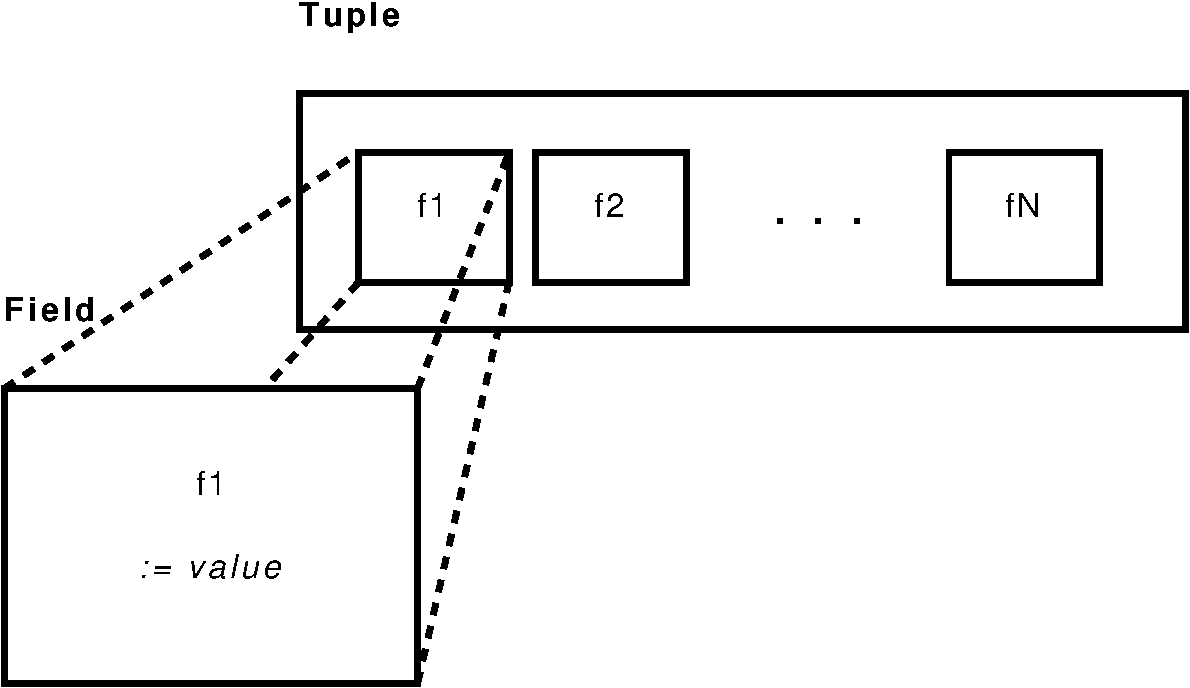
\includegraphics[width=0.7\textwidth]{diagrams/tuple_post}
  \caption[Tuple/Post]{The structure of a \textit{tuple} with \textit{posts}}
  \label{fig:method:tuple_post}
\end{center}
\end{figure}

\section{Summary}
\label{sect:method:summary}
In this chapter the most significant decisions for this project have been
presented and explained in detail. In the next chapter, we will present our
novel methodology for translating XQuery queries to relational algebra, dubbed
``Tainting Dependencies''.
